% !TEX root = main.tex
\chapter{The \lhcb experiment}

The Large Hadron Collider (\lhc) is a circular proton-proton collider at the European Organisation for Nuclear Research \cern.
Along with \atlas, \cms and \alice, the \lhcb experiment is one of the four major experiments at the \lhc.
The experiment is specialized on precision measurements of physics processes involving \bquark- and \cquark-quarks.
Below, first the Large Hadron Collider (\lhc) is briefly described, followed by a more detailed description of the \lhcb detector and its components, based on \cite{Alves:2008zz} and \cite{Aaij:2014jba}.
At the end of this chapter the \lhcb software stack will be described briefly.

\section{The Large Hadron Collider}

\begin{figure}[tbp]
    \centering
    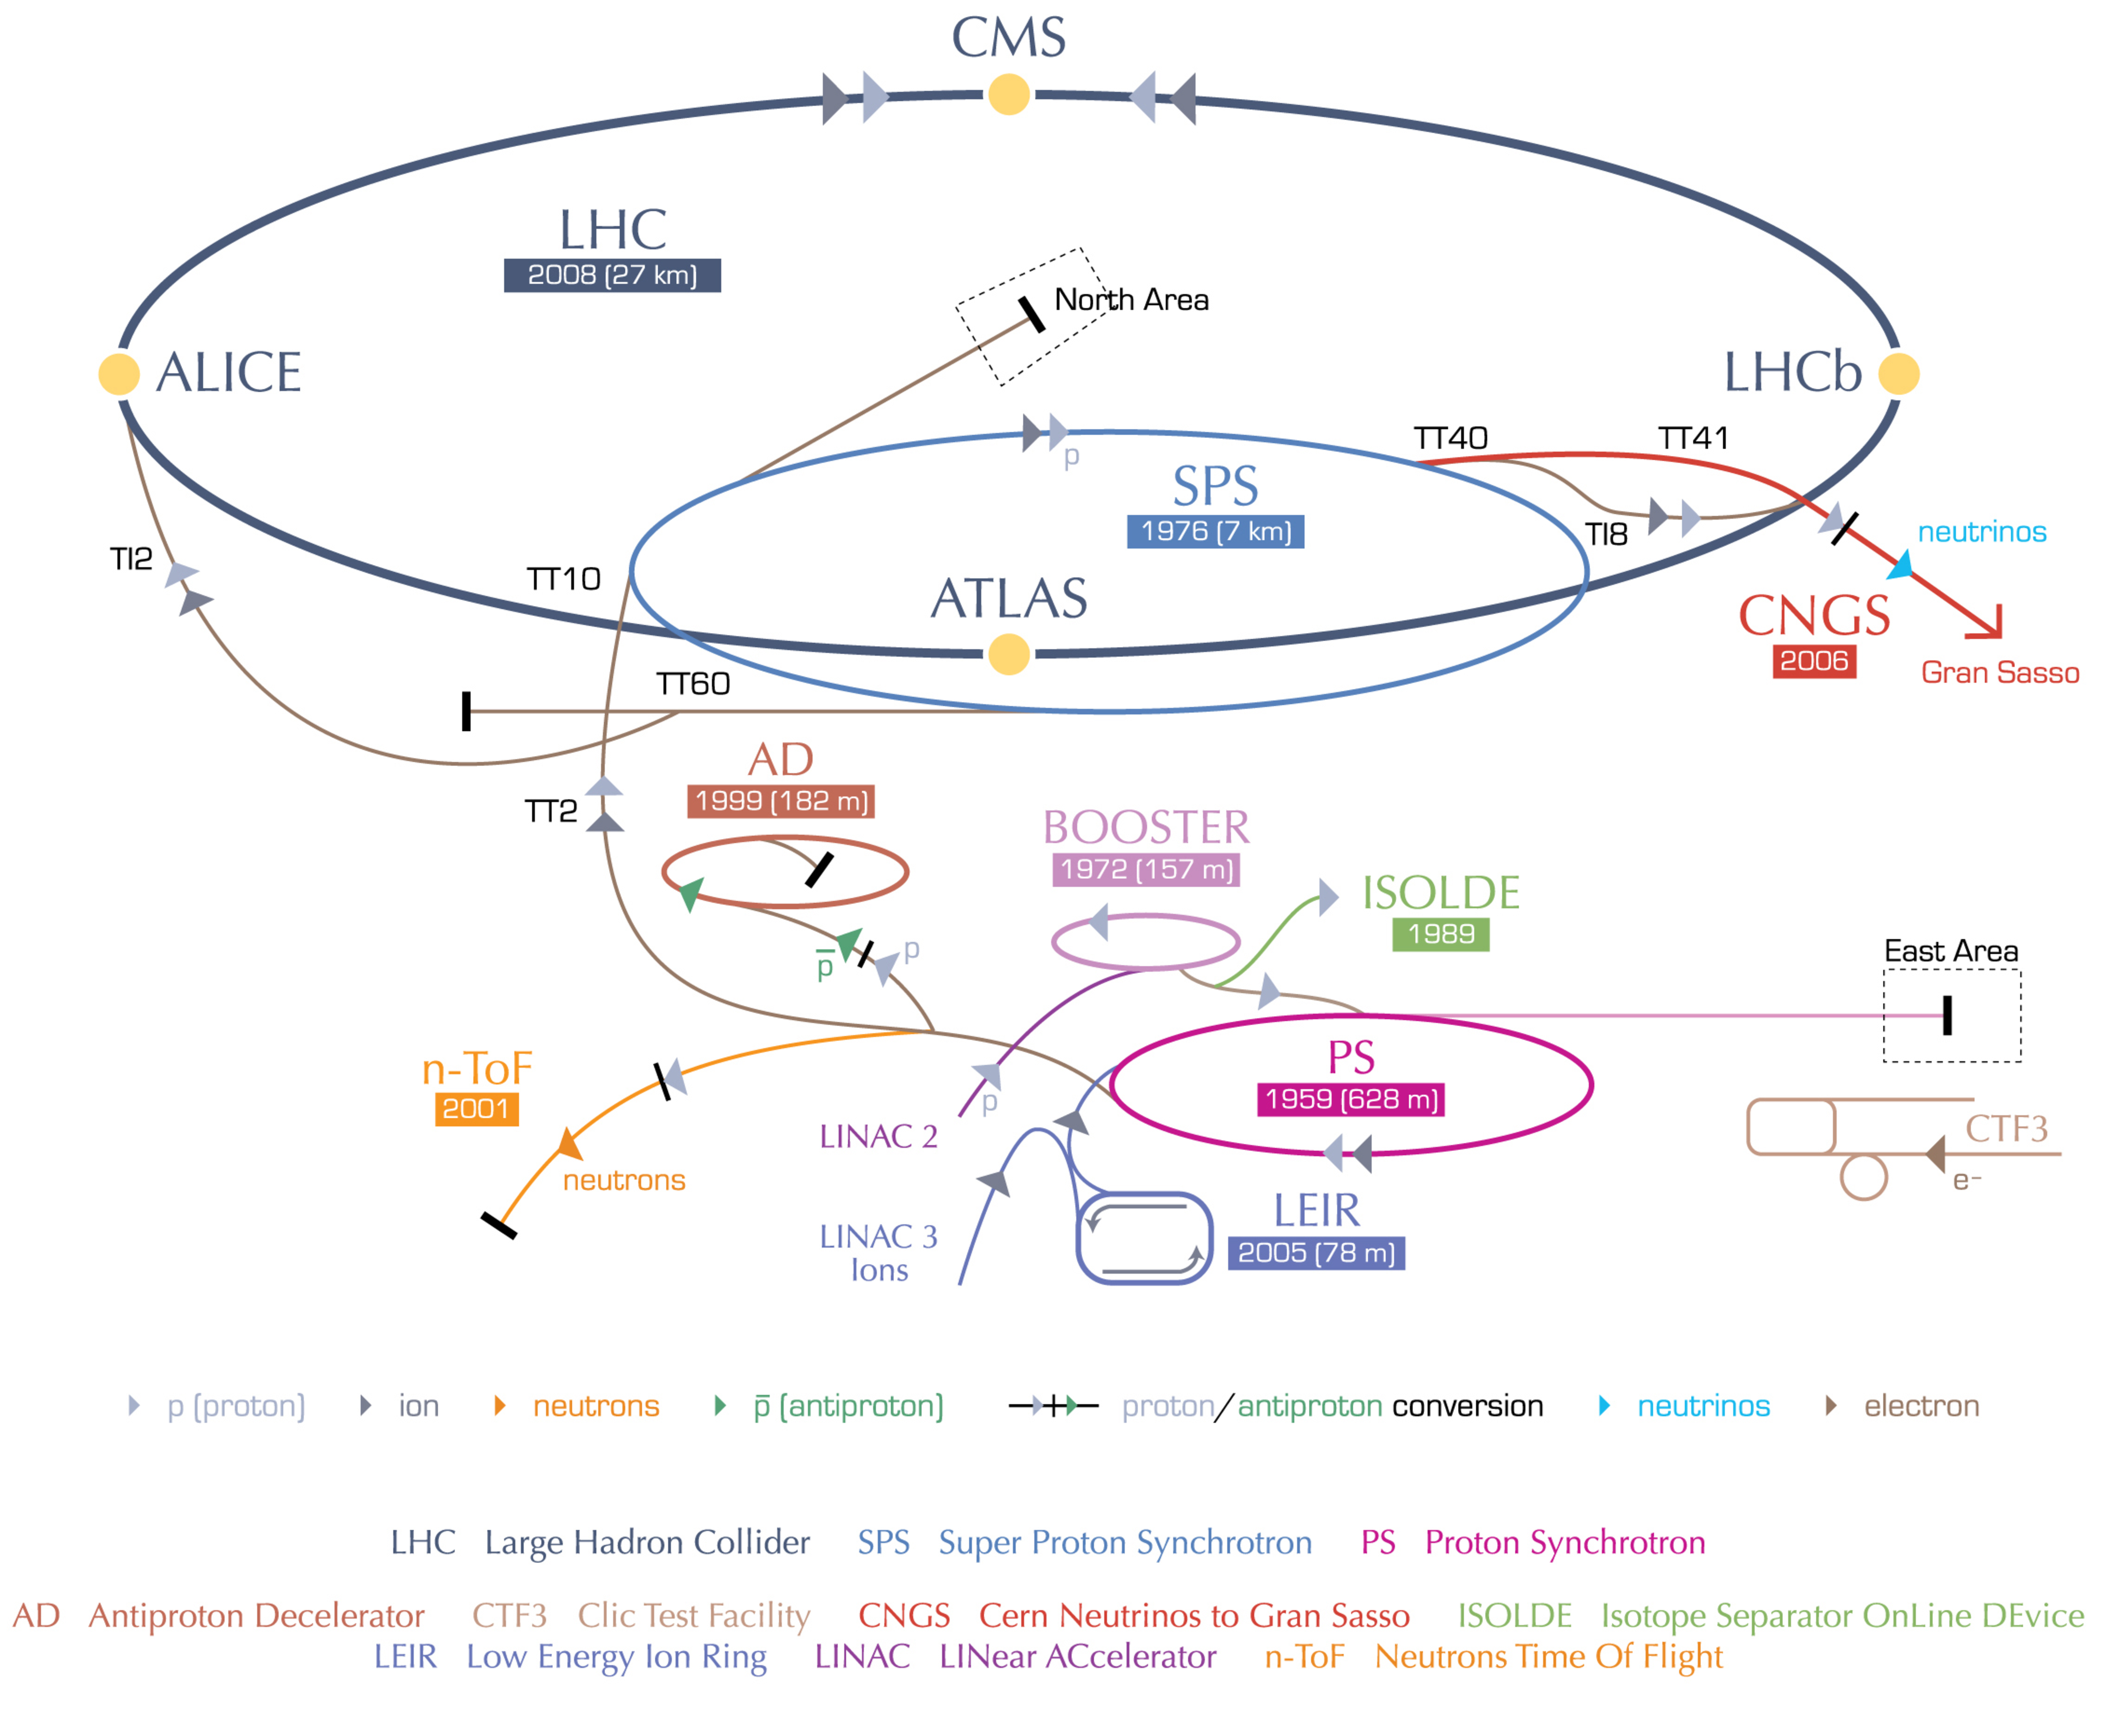
\includegraphics[width=0.75\textwidth]{05lhcb/figs/cern.pdf}
    \caption{Schematic view of the CERN accelerator complex.
    The protons for the LHC are first pre-accelerated to an energy of \SI{450}{\giga\electronvolt} in the LINAC 2, the booster, the proton synchrotron (PS) and the super proton synchrotron (SPS).
    Their path is indicated in the illustration by the light grey arrows~\cite{Christiane:1260465}.}
    \label{fig:CernAccelerators}
\end{figure}
The \lhc is a circular accelerator at \cern near Geneva, Switzerland, with a circumference of about \SI{27}{\kilo\metre}.
It is designed to collide protons at a centre-of-mass energy of up to $\sqrt{s} = \SI{14}{\tera\electronvolt}$ at a luminosity of \SI{e34}{\per\cm\squared\per\second}~\cite{Bruening:782076}.
Two proton beams are accelerated in opposite directions and brought to collision at four points, where the \atlas, \cms and \alice, the \lhcb experiments are located.
The first protons in the \lhc were accelerated in \num{2008}.

The \lhc operates in running periods, the first from \numrange{2010}{2012} (Run I), followed by the long shutdown 1 in \num{2013} and \num{2014}.
During the Run I the proton beams consisted of about \num{1380} proton bunches, colliding at centre-of-mass energies of $\sqrt{s}=\SI{7}{\tera\electronvolt}$ (\num{2010} and \num{2011}) and \SI{8}{\tera\electronvolt} (\num{2012})~\cite{LHC_statistic}.
For the currently ongoing second running period (Run II) the energy and the number of proton bunches per beam were increased to $\sqrt{s}=\SI{13}{\tera\electronvolt}$ and \num{2220}, respectively~\cite{LHC_statistic}.
The latter was achieved by reducing the bunch spacing from \SI{50}{\nano\second} to \SI{25}{\nano\second}.

Before the protons are injected into the \lhc accelerator ring, they have to be pre-accelerated.
This is first done in a linear accelerator, the LINAC 2, followed by the booster, the proton synchrotron (PS) and the super-proton synchrotron (SPS), all of which are circular accelerators.
From the SPS, the protons are then injected into the \lhc ring with an energy of \SI{450}{\giga\electronvolt}~\cite{Bruening:782076} (see \cref{fig:CernAccelerators}).
In order to keep the almost high-energy protons on their circular path, \num{1232} superconducting dipole magnets with a length of \SI{14.3}{\metre} each and a field strength of up to \SI{8.33}{\tesla} are needed.

As already mentioned, four major experiments are located at the \lhc.
\atlas and \cms are multi-purpose experiments collecting data at maximum luminosity, \alice mainly studies quark gluon plasmas.
The fourth experiment, \lhcb, performs primarily precision measurements in the field of flavour physics, especially with \bquark- and \cquark-hadrons.
In contrast to the three other experiments, the detector does not cover the entire spatial angle, but is designed as a forward spectrometer.

\section{The \lhcb detector}

The LHCb detector is a single-arm forward spectrometer with an angular coverage of about \SIrange{10}{250}{\milli\radian}.
The detector geometry is based on the fact that the mainly investigated \bbbar-quark pairs have a high probability of being produced in forward or backward direction (see \cref{fig:anglePlots}).
\begin{figure}[tbp]
    \centering
    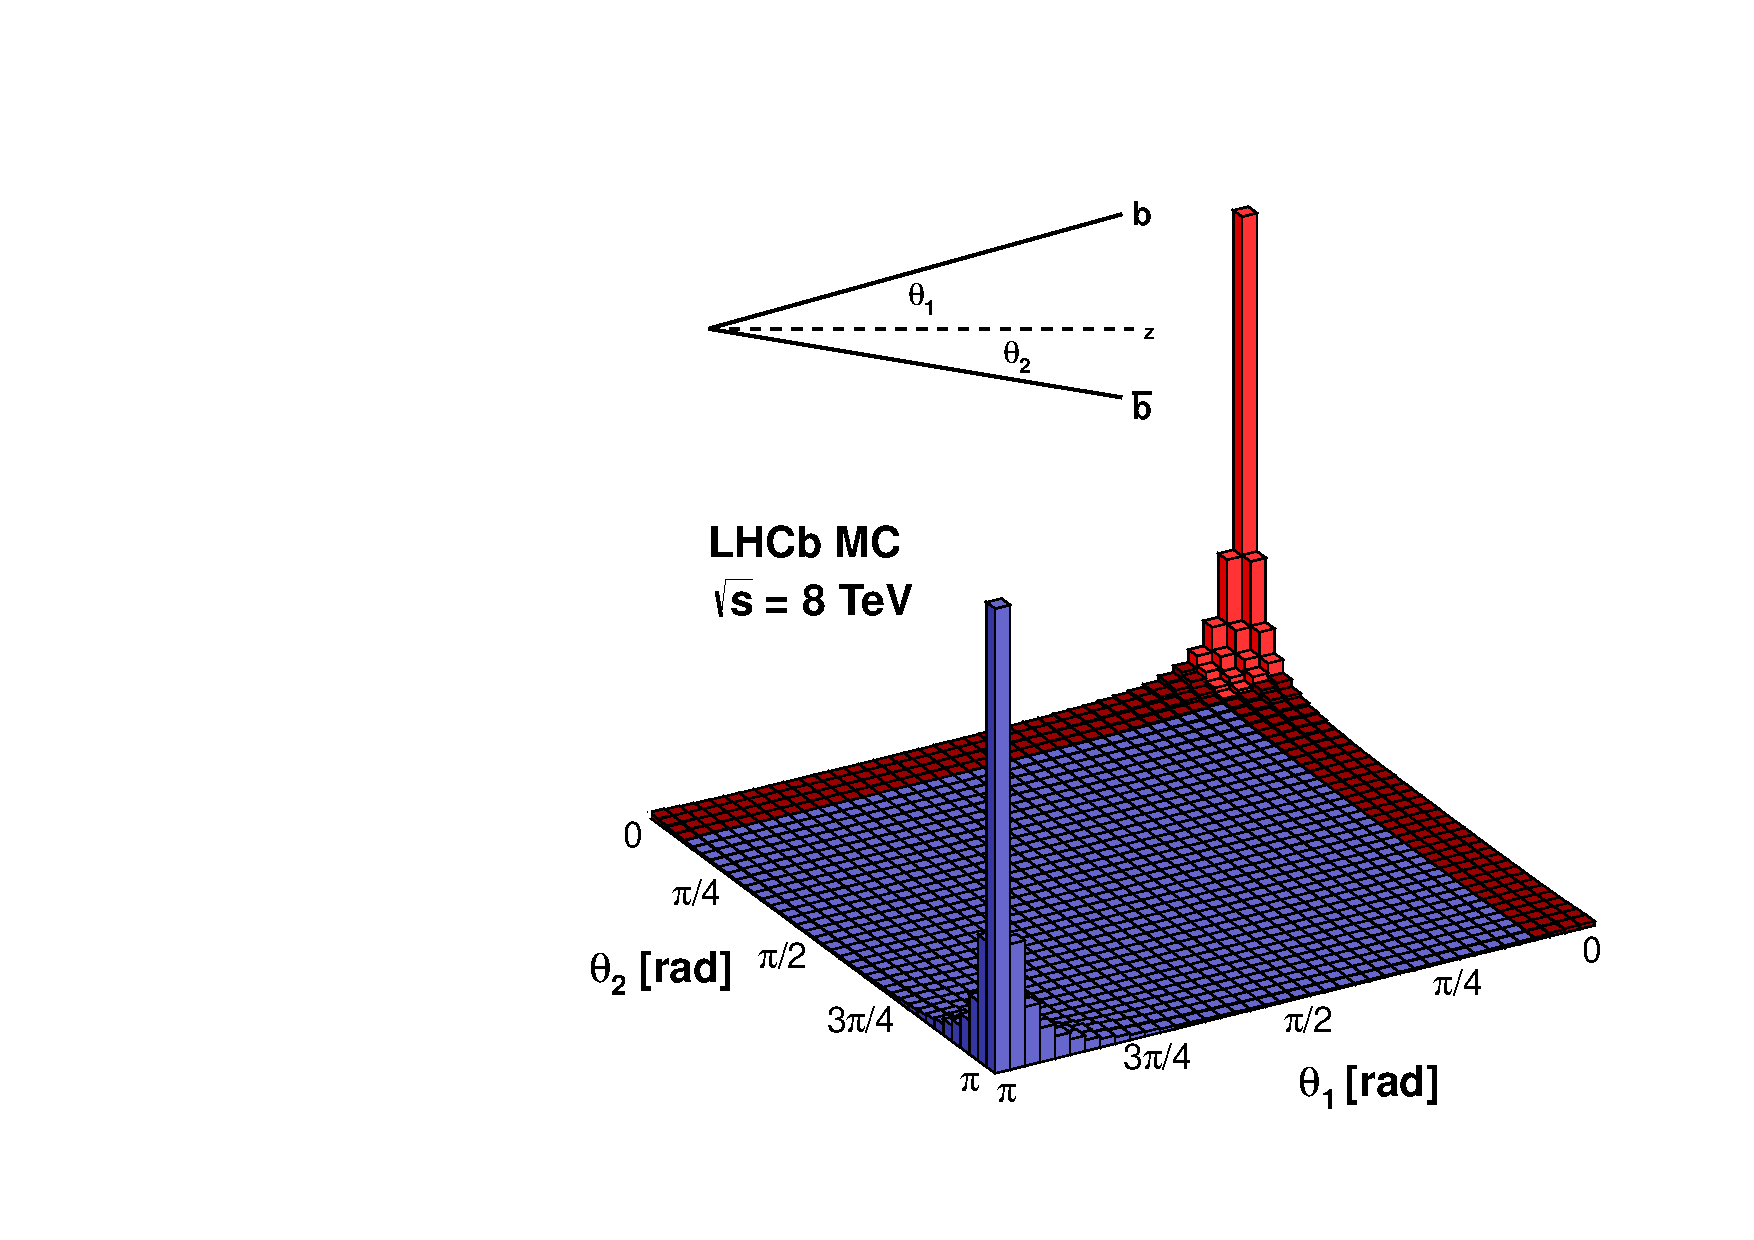
\includegraphics[width=0.4\textwidth]{05lhcb/figs/bbbarCorrelation_angle.pdf}
    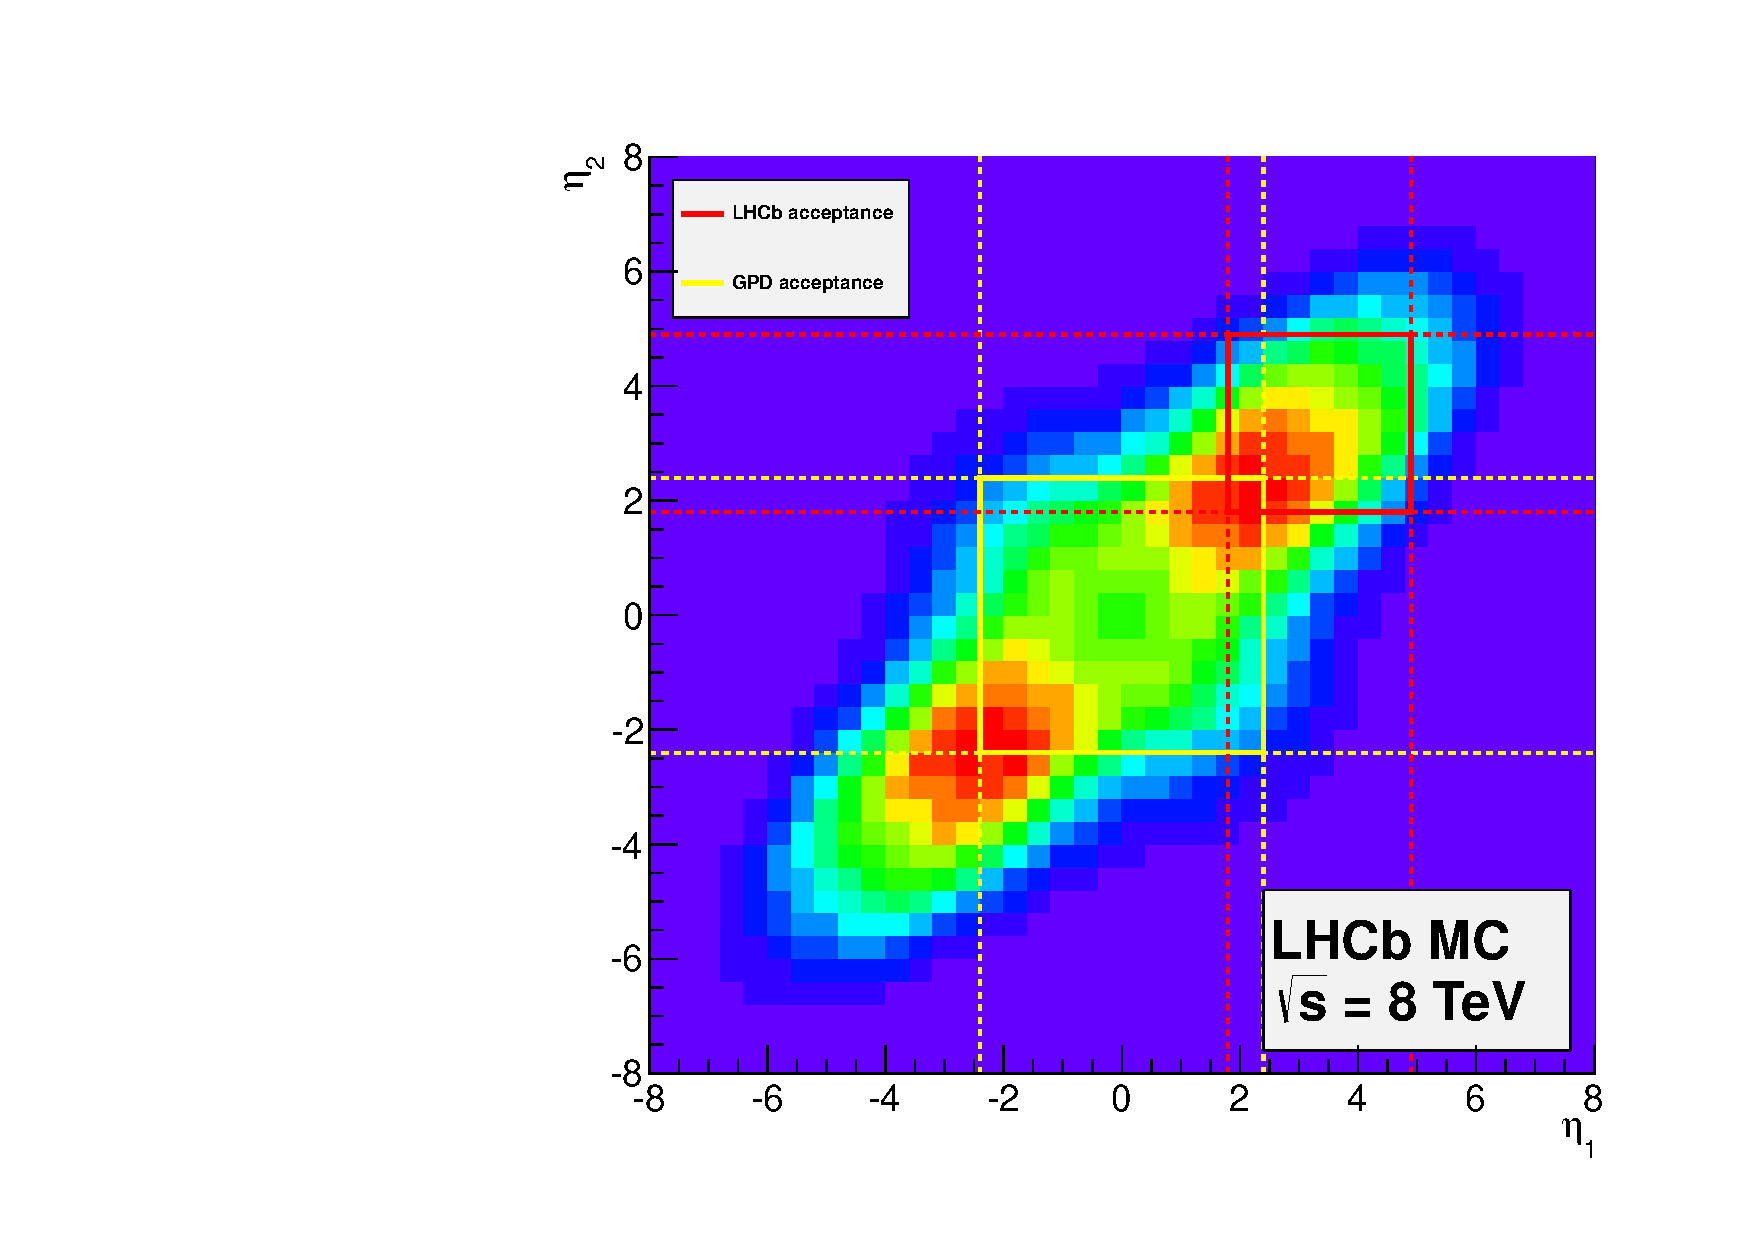
\includegraphics[width=0.4\textwidth]{05lhcb/figs/bbbarCorrelation_rapidity.pdf}
    \caption{Left: Angular distribution of the \bbbar-quark pairs with respect to the beam axis in a proton-proton collision with a centre-of-mass energy of $\sqrt{s}=\SI{8}{\tera\electronvolt}$ as expected from simulations.
    The \lhcb detector acceptance is shown in red.
    Right: Simulated pseudo-rapidity distribution for two \bquark-quarks produced in a proton-proton collision with a centre-of-mass energy of $\sqrt{s}=\SI{8}{\tera\electronvolt}$.
    The yellow box represents the acceptance of a general-purpose detector as \cms or \atlas, the red box shows the \lhcb detector acceptance~\cite{angle_plots}.}
    \label{fig:anglePlots}
\end{figure}
\begin{figure}[tbp]
    \centering
    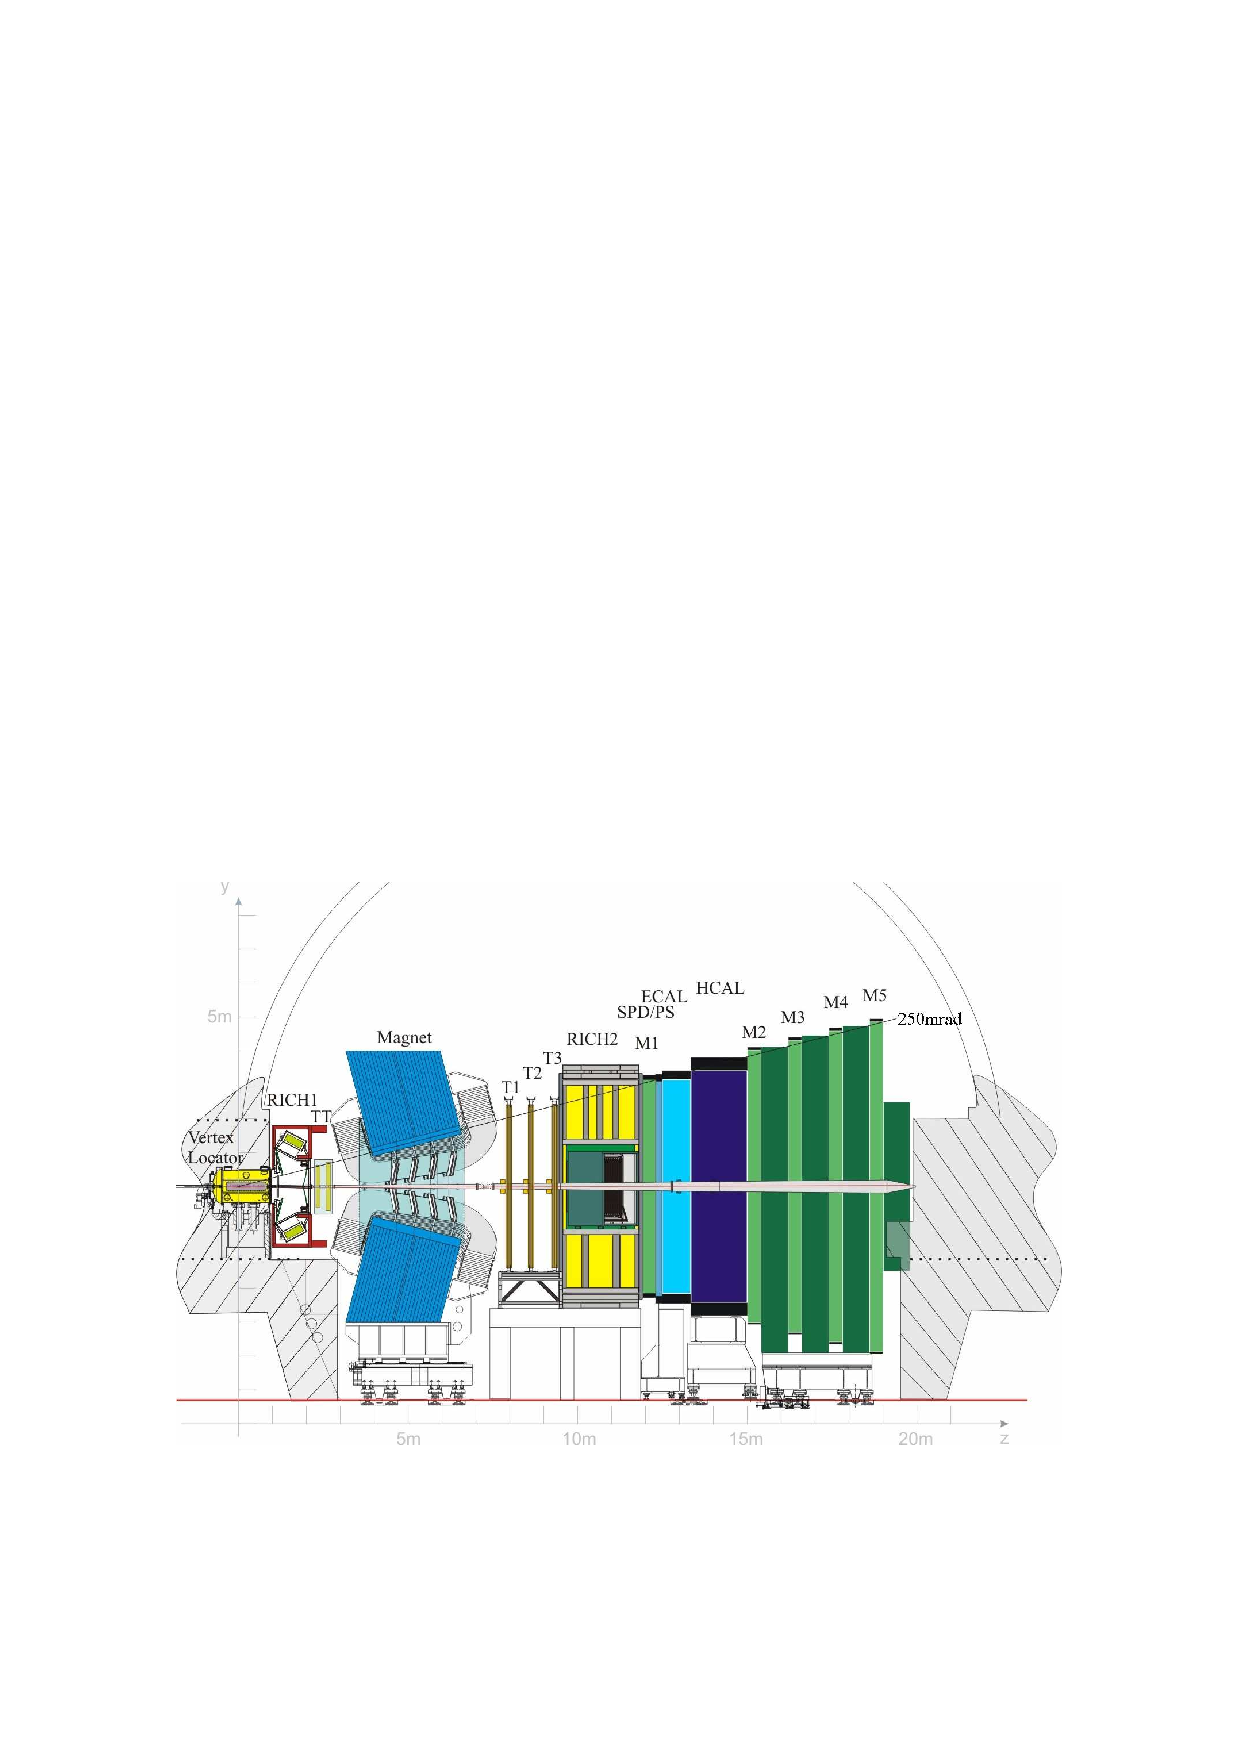
\includegraphics[width=0.8\textwidth]{05lhcb/figs/detector.pdf}
    \caption{Schematic structure of the \lhcb detector: The \velo, the two \rich detectors, as well as the tracking system with magnet, calorimeter and the muon chambers.
    The collision point is located on the left side, enclosed by the \velo~\cite{Alves:2008zz}.}
    \label{fig:lhcbdetector}
\end{figure}
Despite the limited angular coverage, about \SI{25}{\percent} of \bbbar quark pairs are within the detector acceptance.
Furthermore, it is important at \lhcb to resolve individual processes as detailed as possible.
The fewer proton-proton collisions occur simultaneously, the easier this is.
Therefore, \lhcb does not use the maximum luminosity provided by the \lhc, but a constant luminosity of about \SI{4e32}{\per\cm\squared\per\second}~\cite{LHC_statistic}.
This is adjusted by reducing the overlap of the colliding proton bunches in the \lhcb detector compared to the other experiments.
However, since the collision rate with currently \SI{20}{\mega\hertz} is still too high to store all events directly, powerful trigger systems are also required, which already make an initial selection of the data and preserving as many different decay modes as possible.
Furthermore, especially during the injection and accelerating phases of the \lhc beam instabilities may arise which could cause a significant damage in detector components close to the beam pipe.
To protect the detector from such incidents, it is equipped with several safety systems.
The main protection system is the beam conditions monitor (BCM), which measures the particle flux in close vicinity of the beam pipe at two locations downstream and upstream of the \velo~\cite{Ilgner:2010vu}.
As a safety system it is able to remove the beam-permit signal and therefore to dump the \lhc beam.
Accordingly, the BCM is powered by the \lhc-mains through an uninterruptible power supply.

In the following, the individual components of the LHCb detector (see \cref{fig:lhcbdetector}) based on \cite{Alves:2008zz} are explained, separately for the components of the tracking system, the particle identification system and the \lhcb trigger. Though it is important to note, that neither the components described in \cref{sec:tracking} nor the components described in \cref{sec:PartID} are exclusively used for tracking or particle identification purposes, but always a combination of all components is needed for the final reconstruction.

\subsection{The tracking system}
\label{sec:tracking}

The tracking system consists of the \velo, which encloses the collision point, the \ttracker and the tracking stations T1-T3.
Furthermore, a dipole magnet to bend the tracks of charged particles is part of the tracking system.

\subsubsection*{The \velo}
\label{sec:velo}

The vertex locator (\velo) is the detector component closest to the collision point.
It is used to resolve primary and secondary vertices with high precision.
\begin{figure}[tbp]
    \centering
    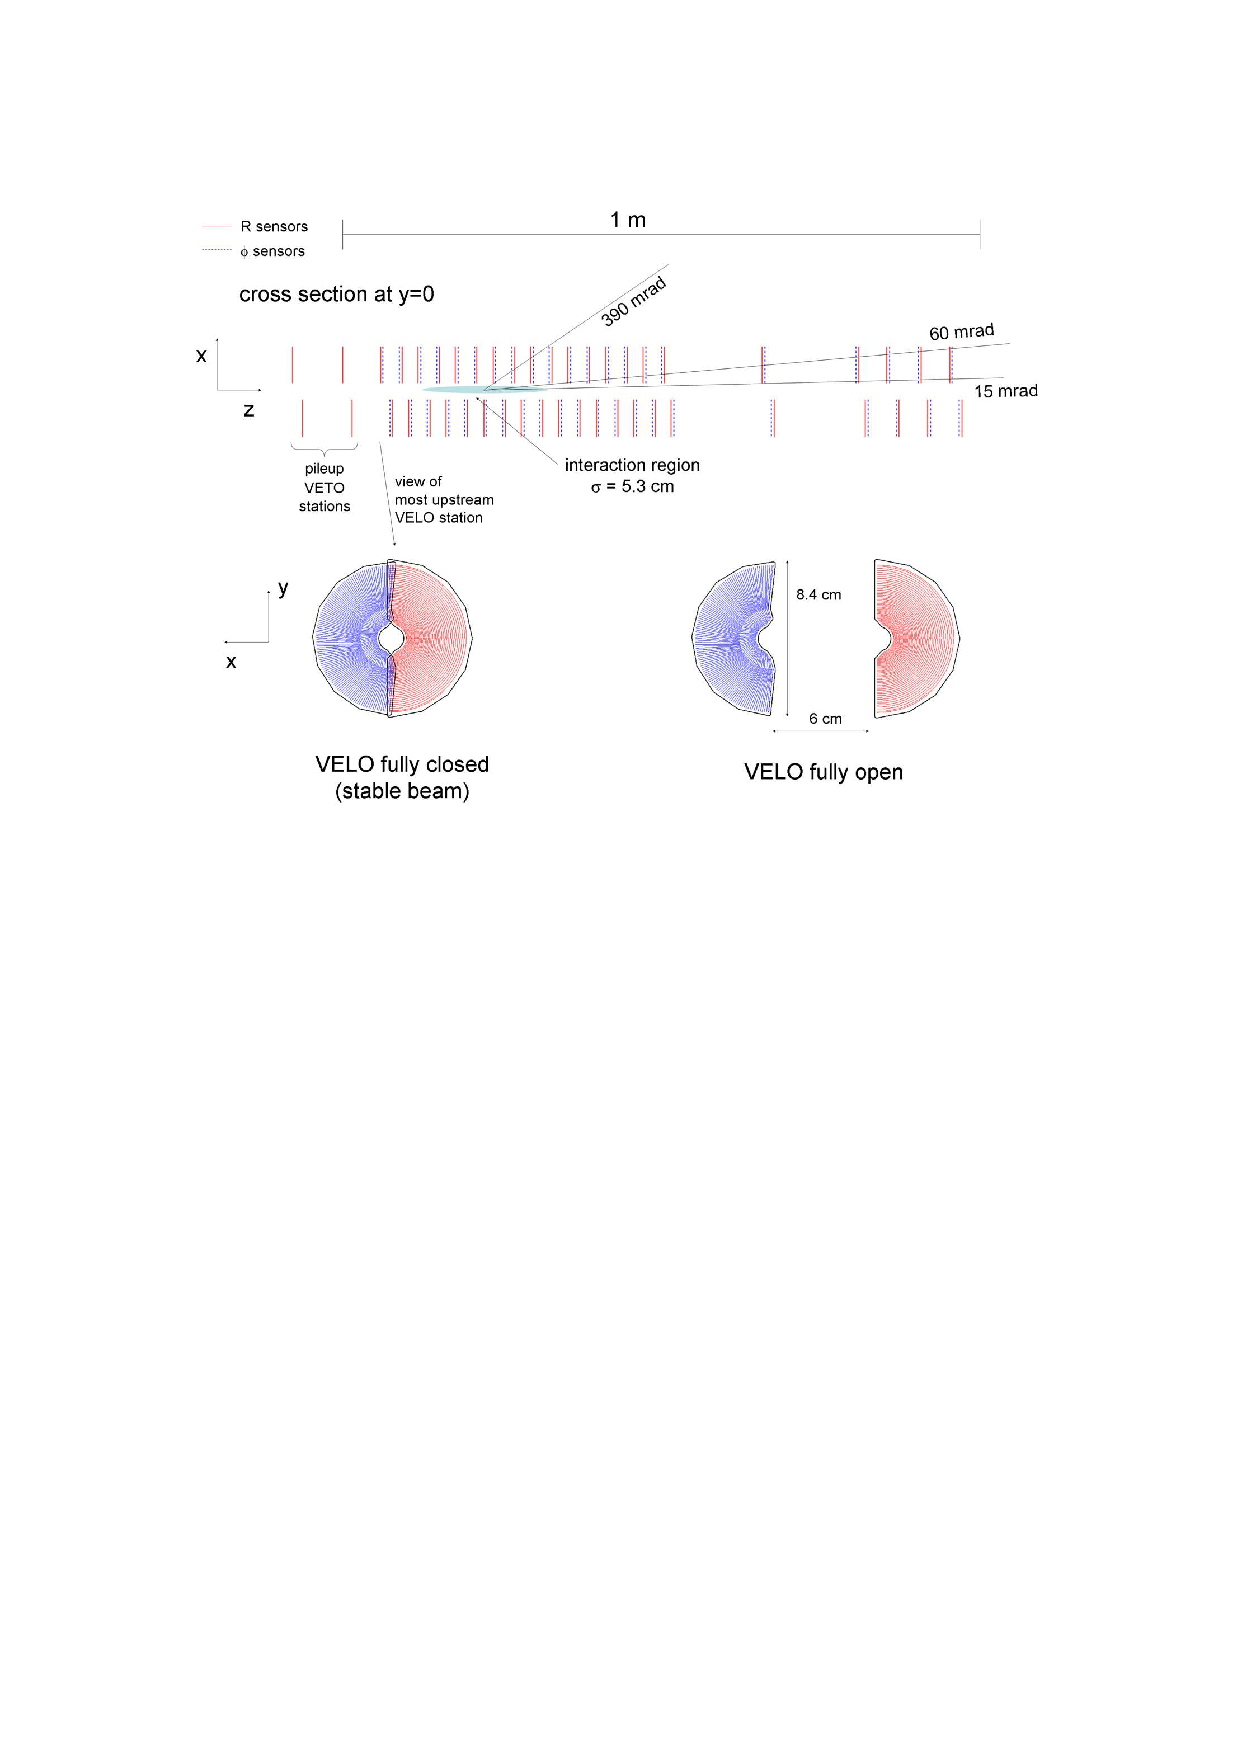
\includegraphics[width=0.75\textwidth]{05lhcb/figs/velo.pdf}
    \caption{Top: View through the $(x,z)$-plane of the \velo at $y=0$ with closed modules.
    Bottom: View from the beam direction onto a module in closed and open state.
    The two halves for $\phi$- (blue) and $r$-measurement (red) can be seen~\cite{Alves:2008zz}.}
    \label{fig:velo}
\end{figure}
The \velo is composed of \num{21} semicircular silicon modules which can be moved up to \SI{8}{\milli\metre} to the beam.
These measure the $r$ and $\phi$ coordinates of the hits left by a traversing charged particle and are mounted along the beam axis as shown in \cref{fig:velo}.
Furthermore, the inner part close to the collision point of the protons is distinguished from an outer part downstream.

To reconstruct a track for a tranversing particle in the \velo it is required that the particle generates hits in at least three stations.
To achieve an angular acceptance of \SI{300}{\milli\radian} of the \velo under this condition, the distance between the inner stations is smaller than \SI{5}{\centi\metre} with a sensor radius of \SI{42}{\milli\metre}.
This small distance leads to a quite short extrapolation distance from the first measured hit to the interaction point.
The resolution of the interaction point, also denoted as \ac{PV}, depends on the number of tracks making the vertex.
For a \ac{PV} with \num{25} tracks the resolution was \SI{13}{\micro\metre} in the $x$ and $y$ coordinates and \SI{71}{\micro\metre} in $z$ in Run I~\cite{Aaij:2014jba}.

For particles, which are created at $z=\SI{10.6}{\centi\metre}$ downstream of the nominal interaction point, the lower limit of the angular accceptance is \SI{15}{\milli\radian}.

To cover full azimuthal acceptance, the two detector halves of each module overlap.
This is possible because the $z$-positions of the respective halves are shifted by \SI{1.5}{\centi\metre} to each other (see \cref{fig:velo}).

\subsubsection*{Tracking stations}
\label{sec:trackingStations}

The tracking stations comprise the Tracker Turicensis (\ttracker) and the three tracking stations T1 to T3 .
The stations T1 to T3 are further divided into an inner area close to the beam pipe, the Inner Tracker (\intr), and more distant areas from the beam pipe, denoted as Outer Tracker (\ot).
A dipole magnet is located between the \ttracker and the tracking station T1 which will be described in \cref{sec:magnet}.
Technologically, the \ttracker and the \intr are silicon trackers (\st).

The \st are made of silicon strips with a width of \SI{200}{\micro\metre}, what leads to spatial resolution of \SI{50}{\micro\metre} in the \intr and the \ttracker.
The \ttracker is directly located upstream of the \richone.
It is \SI{150}{\centi\metre} wide and \SI{130}{\centi\metre} high.
The \intr is installed in the central part around the beam pipe of the three stations T1 to T3.
It covers a region \SI{120}{\centi\metre} wide and \SI{40}{\centi\metre} high as shown in \cref{fig:InnerTracker}.
\begin{figure}[tbp]
    \centering
    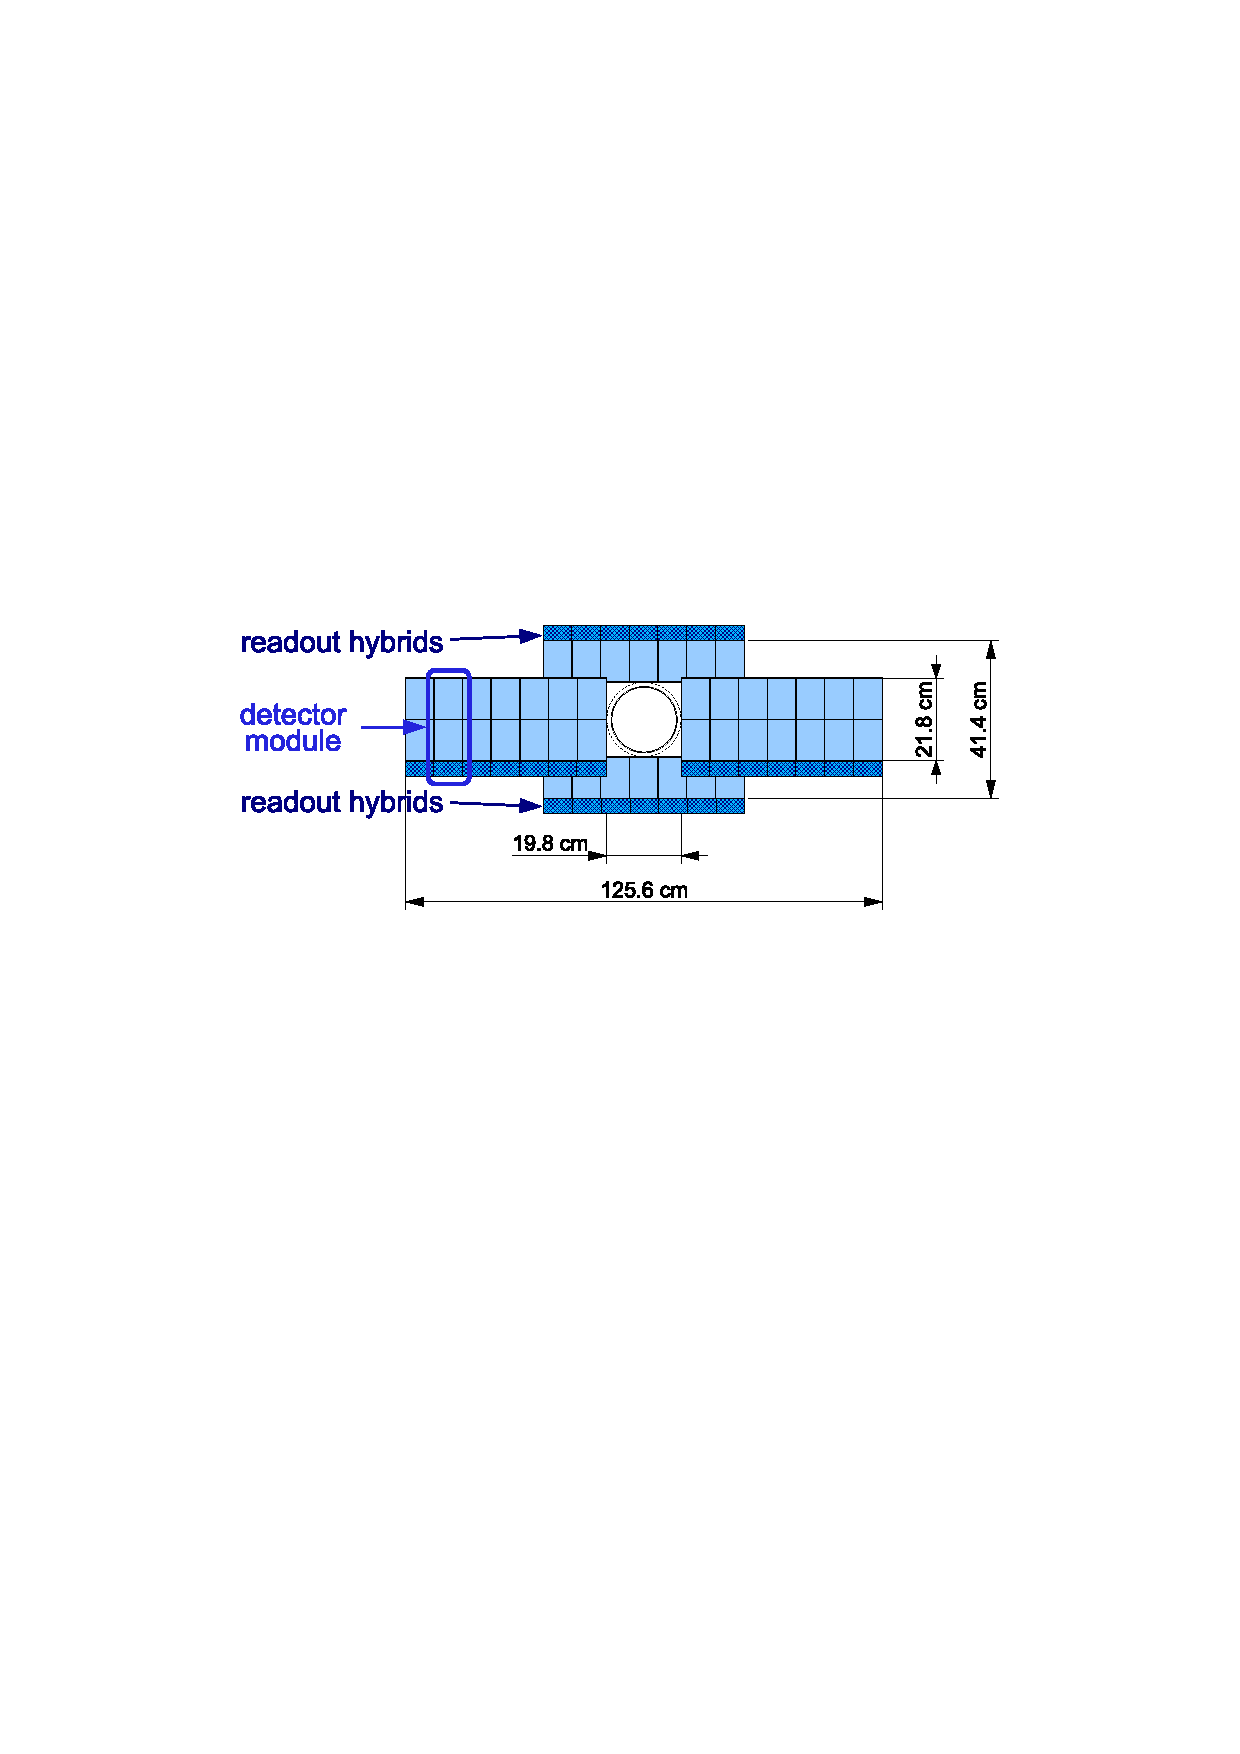
\includegraphics[width=0.75\textwidth]{05lhcb/figs/IT.pdf}
    \caption{Schematic view of a layer of \intr with readout electronics.
    One station consists of four such layers, whereby the middle layers are rotated around the $z$-axis to obtain additional angular information~\cite{Alves:2008zz}.}
    \label{fig:InnerTracker}
\end{figure}

The OT is a detector made of drift tubes filled with gas.
The drift time of ionized gas atoms and their electrons is measured in the drift tubes and from this drift time the ionization spot is determined .
The gas mixture in the drift tubes consists of \SI{70}{\percent} argon, \SI{28.5}{\percent} \cotwo and \SI{1.5}{\percent} $\mathrm O_2$.
This composition guarantees fast drift times of about than \SI{35}{\nano\second} and a high spatial resolution of \SI{205}{\micro\metre}.
The momentum resolution of the \ot is approximately \SI{0.4}{\percent}, with an overall reconstruction efficiency of \SI{80}{\percent}~\cite{Alves:2008zz}.

All tracking stations, \ie both, the \ttracker and the stations T1 to T3, are constructed out of four layers each, with the middle layers rotated by $\pm\SI{5}{\degree}$ around the beam axis so that the $y$-coordinate of a hit, left by a traversing particle, can be determined.

\subsubsection*{The dipole magnet}
\label{sec:magnet}

As mentioned before, the dipole magnet is located between the \ttracker and the tracking station T1.
It covers an acceptance of $\pm\SI{250}{\milli\radian}$ vertically and $\pm\SI{300}{\milli\radian}$ horizontally.
The magnet is designed as a conventional magnet with saddle-shaped coils.
The integrated magnetic field strength is \SI{4}{\tesla\metre} for tracks with a length of \SI{10}{\metre}.
Its strength along the $z$ axis is shown in \cref{fig:MagField}.
Tracks of charged particles are bended with in the accelerator plane ($x$-plane) due to the vertical magnetic field.
\begin{figure}[tbp]
    \centering
    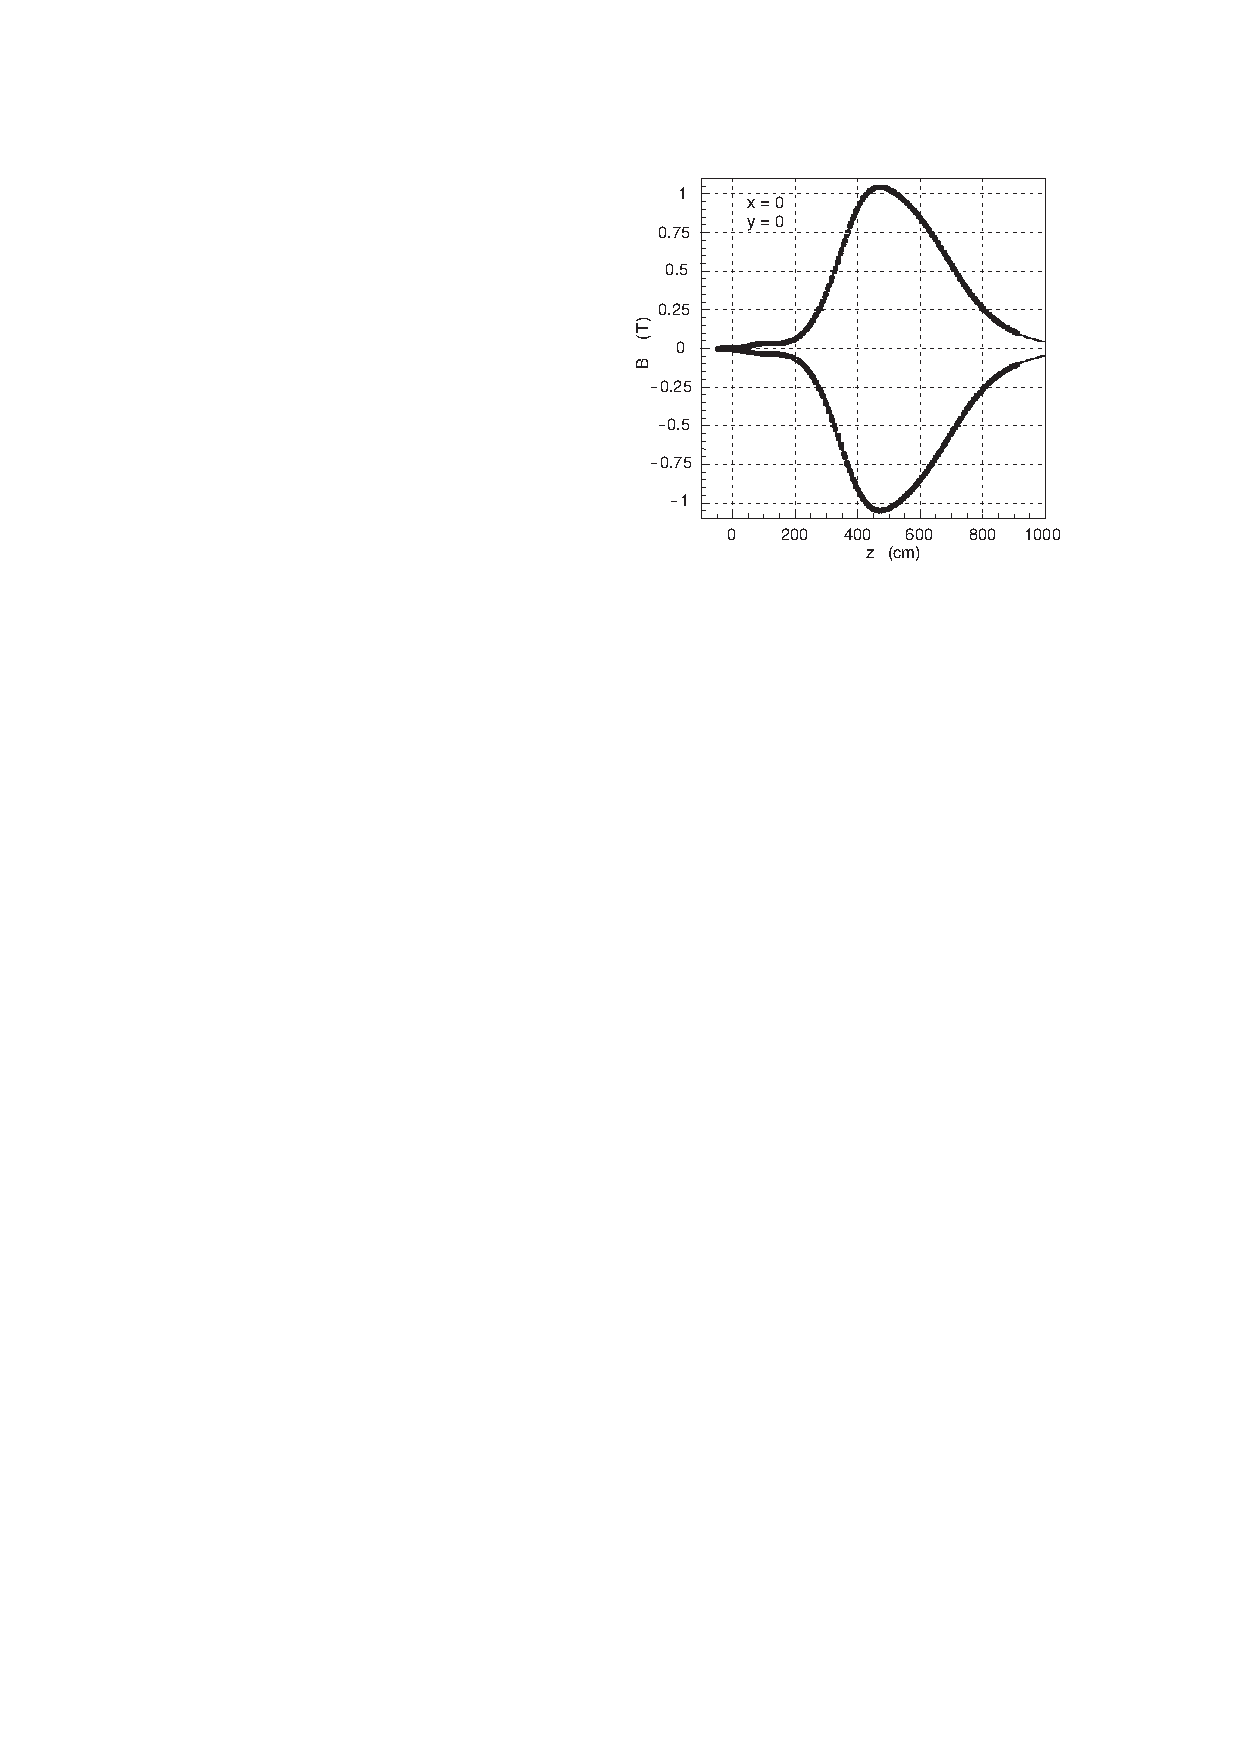
\includegraphics[width=0.5\textwidth]{05lhcb/figs/magnetField.pdf}
    \caption{Magnetic field along the $z$-axis~\cite{Alves:2008zz}.}
    \label{fig:MagField}
\end{figure}
The magnet yoke consists of \SI{100}{\milli\metre} thick laminated low carbon steel plates with a maximum weight of \SI{25}{\tonne}.
The relative precision of the magnetic field needed to achieve the desired momentum resolution is $\mathcal{O}\!\left(10^{-4}\right)$.
During datataking the polarity is inverted regularly to prevent systematic effects due to \eg different performances depending on the area of the detector which the particles traverses.

\subsection{The particle identification system}
\label{sec:PartID}

The particle identification system consists of two \rich detectors, the first downstream of the \velo, the second directly downstream of the tracking station T3.
Further, downstream of the second \rich detector, the electromagnetic and hadronic calorimeters are located, followed by the muon chambers.

\subsubsection*{The \rich detectors}
\label{sec:rich}

An important factor at \lhcb is the particle identification, especially the distinction between pions and kaons.
To realize this, \lhcb has two ring imaging Cherenkov detectors, \richone and \richtwo.
These detectors use the Cherenkov effect, in which particles fly faster through a medium than the speed of light in that medium.
These particles emit electromagnetic radiation with an opening angle $\theta$, where $\theta$ depends on the speed of the particles:
\begin{equation}
\cos\!\left(\theta\right) = \frac{1}{n\beta}.
\end{equation}
Here $n$ is the refractive index of the traversed medium and $\beta = \nicefrac{v}{c}$.
Together with the momentum information from other detector components, different particles can be distuingished.
Since the momentum spectrum changes with the polar angle (angle of a particle to the beam axis), the \rich system consists of the two components \richone and \richtwo.
\richone identifies particles with small momenta of about \SIrange{1}{60}{\giga\electronvolt}~\cite{Alves:2008zz} with a mixture of aerogel and \cfourften, while \richtwo uses a \cffour gas and distinguishes particles with larger momenta in the range of \SIrange{15}{100}{\giga\electronvolt}~\cite{Alves:2008zz}. Because of these different momentum ranges, \richone is located directly behind the \velo, while \richtwo is located downstream of the tracking stations T1 to T3.

Averaging over the momentum, the efficiency to identify a kaon as such is about \SI{95}{\percent} with a pion misidentification rate of about \SI{10}{\percent}. This latter number can be reduced by slightly stricter requirements yielding a pion misidentification rate of about \SI{3}{\percent} at a loss in kaon identification efficiency of about \SI{10}{\percent}~\cite{Aaij:2014jba}.

\subsubsection*{The calorimeters}
\label{sec:calorimeters}

The calorimeters have various functions.
On the one hand they support the $\electron$-, $\gamma$- and hadron identifications, on the other hand they measure particle energies and positions.
They also select candidates for the first trigger stage, the L0 trigger, which makes first decisions already \SI{4}{\second} after a proton-proton interaction.
Overall, the calorimeter setup at \lhcb follows the classical arrangement.
An electromagnetic calorimeter (\ecal) is followed by a hadronic calorimeter (\hcal), where the \ecal is responsible for the $\electron$ identification.

To suppress backgrounds from charged pions, the Preshower (\presh) is installed upstream of the \ecal.
For the trigger, backgrounds from \piz with high transverse energy \et are suppressed by the scintillating pad detector (\spd).
Since the hit density varies by two orders of magnitude over the calorimeter surface, the lateral division of the calorimeters increases closer to the beam pipe (see \cref{fig:calorimeter}).
\begin{figure}[tbp]
    \centering
    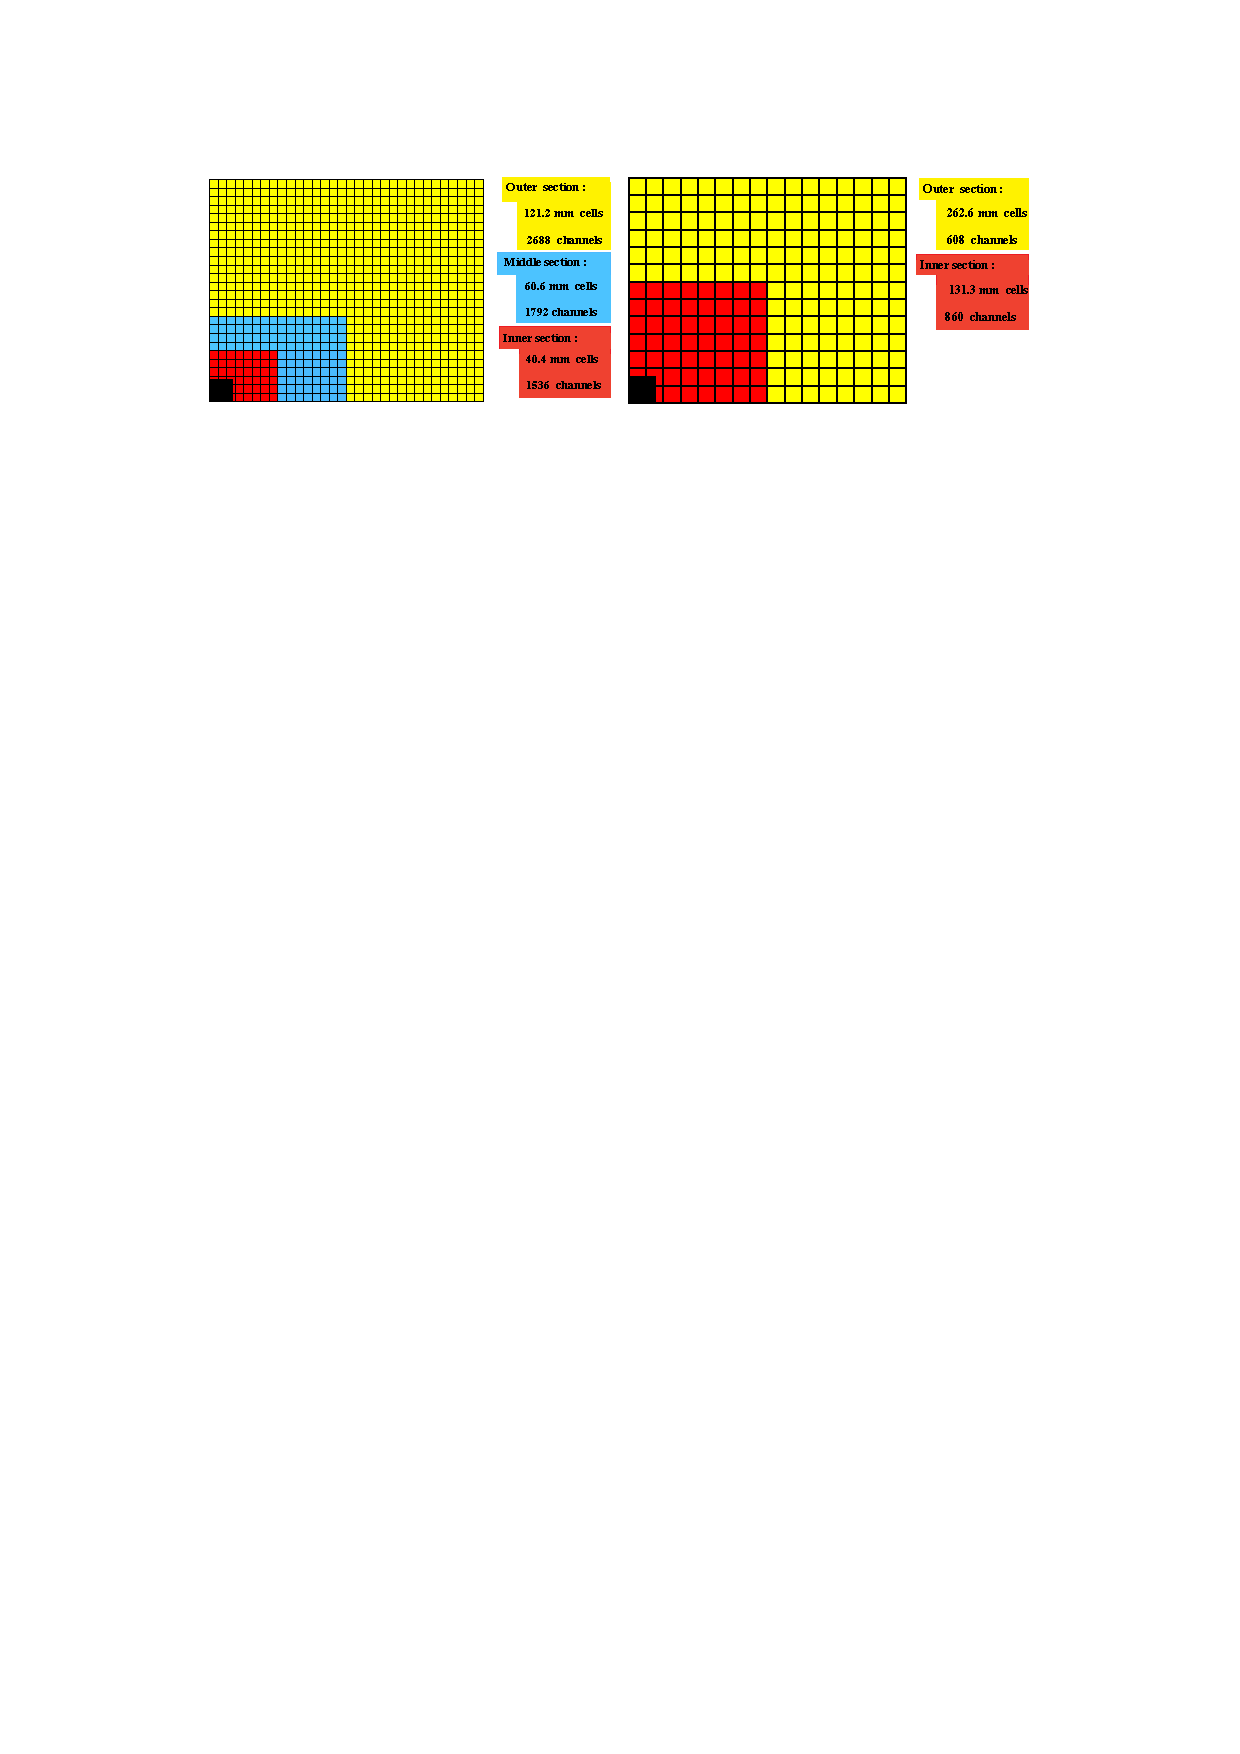
\includegraphics[width=0.9\textwidth]{05lhcb/figs/calorimeter.pdf}
    \caption{Lateral division of the \presh, \spd and \ecal (left) and \hcal (right).
    For all components one quarter of the front view of the detector can be seen.
    The area cut out for the beam pipe is shown in black.~\cite{Alves:2008zz}.}
    \label{fig:calorimeter}
\end{figure}

\subsubsection*{The muon chambers}
\label{sec:muonchambers}

The detection of muons is of fundamental importance at \lhcb.
Both, in many \CP-sensitive decays, such as \BdToJPsiKS, in which the \jpsi is reconstructed in the decay into two muons, and in rare $B$ decays with flavour-changing neutral currents, such as \Bsmm, they can be found in the final states.
There are five muon chambers at \lhcb.
The chamber M1 is located in upstream of the calorimeters, while M2 to M5 are positioned downstream of the \hcal.
The individual stations consist of \SI{80}{\centi\metre} thick iron absorbers, so that the minimum momentum of a muon to pass all five stations must be \SI{6}{\giga\electronvolt}.
Stations M1 to M3 have a relatively high spatial resolution along the $x$-coordinate.
They are mainly used to identify the track directions and to measure the transverse momentum \pt of the muon candidates with a resolution of \SI{20}{\percent}.
The stations M4 and M5 are used for particle identification of traversing muons.

\subsection{Trigger}
\label{sec:trigger}

In contrast to the multipurpose experiments \atlas and \cms, the \lhcb experiment does not operate at the maximum luminosity of $L=\SI{7e33}{\per\centi\metre\squared\per\second}$ provided by the \lhc in Run I, but at a luminosity of $L=\SI{4e32}{\per\centi\metre\squared\per\second}$, in order to ideally record exactly one proton-proton interaction per bunch crossing.
Nevertheless, the data rate must still be reduced from about \SI{20}{\mega\hertz} to about \SI{4}{\kilo\hertz} in order to be stored.
Two trigger stages are available for this purpose: The first stage (L0) works synchronously to the interaction rate of \SI{40}{\mega\hertz} and reduces it to \SI{1}{\mega\hertz}, whereupon the second trigger stage, the high-level trigger (HLT), processes the data independently of the interaction rate.
At a luminosity of $L=\SI{4e32}{\per\centi\metre\squared\per\second}$, events containing a $B$ meson are generated at a rate of about \SI{15}{\kilo\hertz}.
Furthermore, many partial decay widths of the $B$ mesons are smaller than \num{e-3}, so that the trigger system is optimized to select these interesting decays for subsequent analyses with maximum efficiency, while the backgrounds created in the hadronic environment at the \lhc are suppressed to the maximum.

The Level 0 trigger is a pure hardware trigger.
It identifies hadrons, electrons and photons which have maximum transverse energies \et, as well as the two muons with the highest transverse momenta \pt.
The L0 consists of three components: A L0 pile-up system, the L0 calorimeter trigger and the L0 muon trigger.
The aim of the pile-up system is to distinguish between events with one or more visible proton-proton interactions.
The calorimeter and muon components search for the maximum \et or \pt for the corresponding particles.

The HLT is a C++ application and runs on the Event Filter Farm (EFF), a large-capacity computer at \cern.
Every application has full access to all information of an event.
Hence, selection steps could already be applied out here in principle.
However, since the data rate coming from the L0 trigger is very high, the HLT consists of two stages.
The HLT1 reconstructs the partial candidates in the \velo and in the tracking stations, which the L0 transfers.
In addition for photons and neutral pions the absence of charged particles that could be associated with these candidates is confirmed.
Overall, the HLT1 has the task of reducing the data rate to such an extent that a full full pattern recognition is possible in the next step, the HLT2.
At a sufficiently low data rate, in some cases the HLT2 then even reconstructs specific $B$ decays .

\section{The LHCb software stack}

\begin{figure}[tbp]
    \centering
    \includestandalone{05lhcb/figs/LHCbSoftware}
    \caption{Sequence of data processing within the \lhcb software.
    In red the steps to simulate data, in blue the processing of real data is shown.
    The software packages are displayed in rectangles, the transferred data formats in circles.}
    \label{fig:lhcbsoftware}
\end{figure}
The \lhcb software is based on the \gaudi framework~\cite{Barrand:2001ny}, in which different software packages are executed.
The order in which the various packages are executed is shown in \cref{fig:lhcbsoftware}.
The first action on the data recorded by the detector happens in the HLT through the software package \moore \cite{Aaij:2012me, Albrecht:2013fba}, as described in \cref{sec:trigger},.
Afterwards the raw data is reconstructed in \brunel \cite{Szumlak:2007zz, VanderEijk:2001wqa, Kucharczyk:1756296} and the particles are combined in so-called protoparticles.
These protoparticles contain track information and particle identification (PID) information of the concerning particle.
The data is then available as so-called Data Summary Tape Files (DST's) and is further processed for analysis in \davinci.
In the \davinci software project a first preselection (stripping) takes place and the final reconstruction of the different decays is done.
After the stripping, the data has the form of so-called nTuples, which can be analysed by individual analysts.

The generation and simulation of events within the \lhcb detector is implemented in the \gauss package.
The proton-proton-collisions and the hadronisation process are generated using \pythia \cite{pythia6, pythia8}, which runs with a special \lhcb configuration \cite{LHCb-PROC-2010-056}.
Decays and the interaction with the detector are then simulated using the \evtgen \cite{evtgen} and \geant \cite{geant1, geant2} packages, respectively.
This is followed by the \boole project, in which the data is digitized so it can then be further processed as the raw data collected by the detecor.
Furthermore, the generated information (truth information) is stored and can be retrieved after the simulated events have been processed.
Thus, in addition to the detector response, the initially generated states are also known for simulated events.
